\documentclass[12pt]{article}
\usepackage{amssymb,amsmath,cite,geometry,graphicx,url,cleveref}
\addtolength{\textheight}{.8in}
\addtolength{\textwidth}{.9in}
\addtolength{\topmargin}{-.4in}
\addtolength{\evensidemargin}{-.45in}
\addtolength{\oddsidemargin}{-.45in}

\catcode`\@=11

%       This causes equations to be numbered by section

\@addtoreset{equation}{section}
\def\theequation{\arabic{section}.\arabic{equation}}

%       reset section commands

\catcode`\@=11
\def\thesection{\arabic{section}.}
\def\thesubsection{\arabic{subsection}.}
\def\thesubsubsection{\arabic{subsubsection}.}
\def\appendix{\setcounter{section}{0}
        \def\thesection{Appendix.}
        \def\theequation{\Alph{section}.\arabic{equation}}}
\def\section{\@startsection{section}{1}{\z@}{3.5ex plus 1ex minus
   .2ex}{2.3ex plus .2ex}{\large\bf}}

%      reset footnotes

\renewcommand{\thefootnote}{\fnsymbol{footnote}}
\long\def\@makefntext#1{\parindent 0cm\noindent
\hbox to 1em{\hss$^{\@thefnmark}$}#1}

% Different font in captions
\newcommand{\captionfonts}{\small}
\makeatletter  % Allow the use of @ in command names
\long\def\@makecaption#1#2{%
  \vskip\abovecaptionskip
  \sbox\@tempboxa{{\captionfonts #1: #2}}%
  \ifdim \wd\@tempboxa >\hsize
    {\captionfonts #1: #2\par}
  \else
    \hbox to\hsize{\hfil\box\@tempboxa\hfil}%
  \fi
  \vskip\belowcaptionskip}
\makeatother   % Cancel the effect of \makeatletter

\begin{document}
\begin{titlepage}
\vspace{.5in}
\begin{flushright}
June 2018\\  %date
\end{flushright}
\vspace{.3in}

\begin{center}
{\Large\bf
 Efficient Causal Dynamical Triangulations}\\  %title
\vspace{.4in}
{A.~G{\sc etchell}\footnote{\it email: acgetchell@ucdavis.edu}\\
       {\small\it Department of Physics}\\
       {\small\it Univeristy of California}\\
       {\small\it Davis, CA 95616}\\{\small\it USA}}\\[2ex]
\end{center}

\vspace{.3in}
\begin{center}
{\large\bf Abstract}
\end{center}
\vspace*{.1ex}
\begin{center}
\begin{minipage}{4.9in}
{\small
I review constructing piecewise simplicial manifolds using efficient
methods for constructing Delaunay triangulations. I then evaluate the use of
the Metropolis-Hastings algorithm in the Causal Dynamical triangulations
program. I highlight inefficiencies and propose solutions.
}
\end{minipage}
\end{center}
\end{titlepage}
\addtocounter{footnote}{-2}

\section{Introduction}

\begin{quote}
  Nevertheless, due to the inneratomic (sic) movements of electrons, atoms would have to radiate
  not only electromagnetic but also gravitational energy, if only in tiny amounts.
  As this is hardly true in nature, it appears that quantum theory would have to modify
  not only Maxwellian electrodynamics, but also the new theory of gravitation.\cite{einstein_volume_nodate}

  --Einstein, 1916 {\it Approximative Integration of the Field Equations of Gravitation, p.209}
\end{quote}

Quantum gravity is, perhaps, the preeminent hard problem\cite{steve_carlip_why_2014} remaining in theoretical physics, and has been worked on for many years\cite{rovelli_notes_2000}.

Although difficult to test experimentally, a quantum theory of gravity appears to be the key to resolving several important
questions, such as the black hole information paradox.\cite{preskill_black_1992}

Causal Dynamical Triangulations (CDT) \cite{j._ambjorn_dynamically_2001} is a useful approach to
quantum gravity. It is based on the Regge action\cite{regge_general_1961}, which describes General Relativity on simplicial manifolds similarly to the Einstein-Hilbert action on differentiable manifolds.

Using the Metropolis-Hasting algorithm, in the class of Markov Chain Monte Carlo methods (MCMC), unlike other methods it allows
for the analysis of complex distributions in higher dimensions. Better still, in calculating the path integral as a ratio, it allows
the factoring out of terms that we would have a hard time of finding out.

Nevetheless, MCMC algorithms suffer from known problems such as exponentially long convergence times to stationary distributions and sensitivity to step size.

Methods such as slice sampling, Hamiltonian Monte Carlo, and Simulated Annealing are other methods that may be used instead of MCMC.
But each has respective drawbacks:

Slice sampling requires that the sample is evaluatable, which is not always possible. It also runs into difficulties at higher dimensions.

Hamiltonian Monte Carlo (HMC) computes expectations by exploring a continuous parameter space of probability distributions.\cite{betancourt_conceptual_2017}. In certain implementations
it has been show to be extremely fast and efficient\cite{hoffman_no-u-turn_2011}, but it's not necessarily clear how to set this up for the Regge action. Additionally, the parameters may be hard to tune, and it does not handle multimodality well, which is an expected output of quantum gravity ("crumpled or polymer" phase and "other phase of CDT"). Nontheless, I think this is a worthwhile possiblity worth exploring in a future paper.

Like HMC, Simulated Annealing also requires a global parameter space to optimize.\cite{busetti_simulated_nodate} Implementing this in the context of CDT has not, to my knowledge, been explored.

\section{Background}

The Einstein equation describes the curvature of spacetime $R_{\mu\nu}$ in terms of the stress-energy-momentum tensor $T_{\mu\nu}$:

\begin{align}
  R_{\mu\nu}-\frac{1}{2}Rg_{\mu\nu}=8\pi G_{N}T_{\mu\nu}
\end{align}

The Reimann tensor is given by:

\begin{align}
  R_{\sigma\mu\nu}^{\rho}=\partial_{\mu}\Gamma_{\nu\sigma}^{\rho}-\partial_{\nu}\Gamma_{\mu\sigma}^{\rho}+\Gamma_{\mu\lambda}^{\rho}\Gamma_{\nu\sigma}^{\lambda}-\Gamma_{\nu\lambda}^{\rho}\Gamma_{\mu\sigma}^{\lambda}
\end{align}

Where the Affine connection $\Gamma_{\mu\nu}^{\lambda}$ is defined by:

\begin{align}
  \Gamma_{\mu\nu}^{\lambda}=\frac{1}{2}g^{\lambda\sigma}\left(\partial_{\mu}g_{\nu\sigma}+\partial_{\nu}g_{\sigma\mu}-\partial_{\sigma}g_{\mu\nu}\right)
\end{align}

And the (cylindrically symmetric) metric is:

\begin{align}
  g_{\mu\nu}=\left(\begin{array}{cccc}
    e^{2\lambda} & 0 & 0 & 0\\
    0 & -e^{2\left(\nu-\lambda\right)} & 0 & 0\\
    0 & 0 & -e^{2\left(\nu-\lambda\right)} & 0\\
    0 & 0 & 0 & -\frac{r^{2}}{e^{2\lambda}}
    \end{array}\right)
\end{align}
$R^{\rho}_{\sigma\mu\nu}$ can be thought of as encapsulating the intrinsic curvature (see \Cref{parallel-transport-figure}).
\begin{figure}
  \centering
  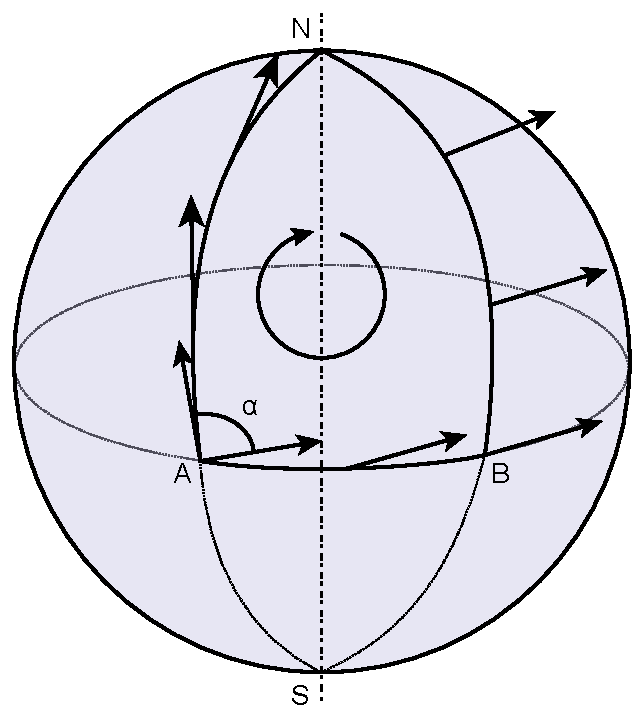
\includegraphics[width=2in]{Parallel_Transport.pdf}
  \caption{Parallel Transport on a spherical surface by Fred the Oyster, CC BY-SA 4.0, https://commons.wikimedia.org/w/index.php?curid=35124171 \label{parallel-transport-figure}}
\end{figure}

From the Reimann tensor one obtains the Ricci tensor using $R_{\mu\nu}=R^{\rho}_{\mu\rho\nu}$, and likewise the Ricci scalar is $R=R^{\mu}_{\mu}$ using the Einstein summation convention.

Given the Ricci scalar the Einstein-Hilbert action is:

\begin{align}
I_{EH}=\frac{1}{16\pi G_{N}}\int d^{4}x\sqrt{-g}(R-2\Lambda)
\end{align}

Where $G_{N}$ is Newton's Gravitational constant and $\Lambda$ is the cosmological constant.

Extremizing the Einstein-Hilbert action produces the equations of motion.

\begin{align}
  \partial I_{EH} = 0 \rightarrow R_{\mu\nu}-\frac{1}{2}Rg_{\mu\nu}=8\pi G_{N}T_{\mu\nu}
\end{align}

In quantum mechanics, one is interested in the transition probability amplitude $\langle B|T|A\rangle$, which is the conditional probability of being in state $B$ given previously being in state $A$. This is generally computed using the path integral.

\begin{align}
  \langle B|T|A\rangle=\int\mathcal{D}[g]e^{iI_{EH}}
\end{align}

Such path integrals are typically not directly computable, for a number of reasons. Quantum Field Theory uses perturbative summation techniques such as Feynman diagrams, but these require a notion of renormalizability for various infinite divergences, and gravity has been shown to be definitively non-renormalizable.\cite{shomer_pedagogical_2007}

In 1961 Regge developed his calculus replacing smooth differentiable manifolds with simplicial manifolds, obeying the following two properties\\[-4ex]
\begin{enumerate}\addtolength{\itemsep}{-1.5ex}
\item close: every $(n-1)$-dimensional subsimplex of a simplex in the manifold is also in the manifold;  
\item connectivity: two connected $n$-dimensional simplices share one and only one $(n-1)$-dimensional subsimplex;
\end{enumerate}
\vspace*{-1ex}

From here on, simplicial manifolds will be referred to as triangulations. Of special note are Delaunay Triangulations, which are well-behaved simplicial manifolds
with a circumsphere property of member simplices which may be seen intuitively in \Cref{DT}.

\begin{figure}
  \begin{center}
  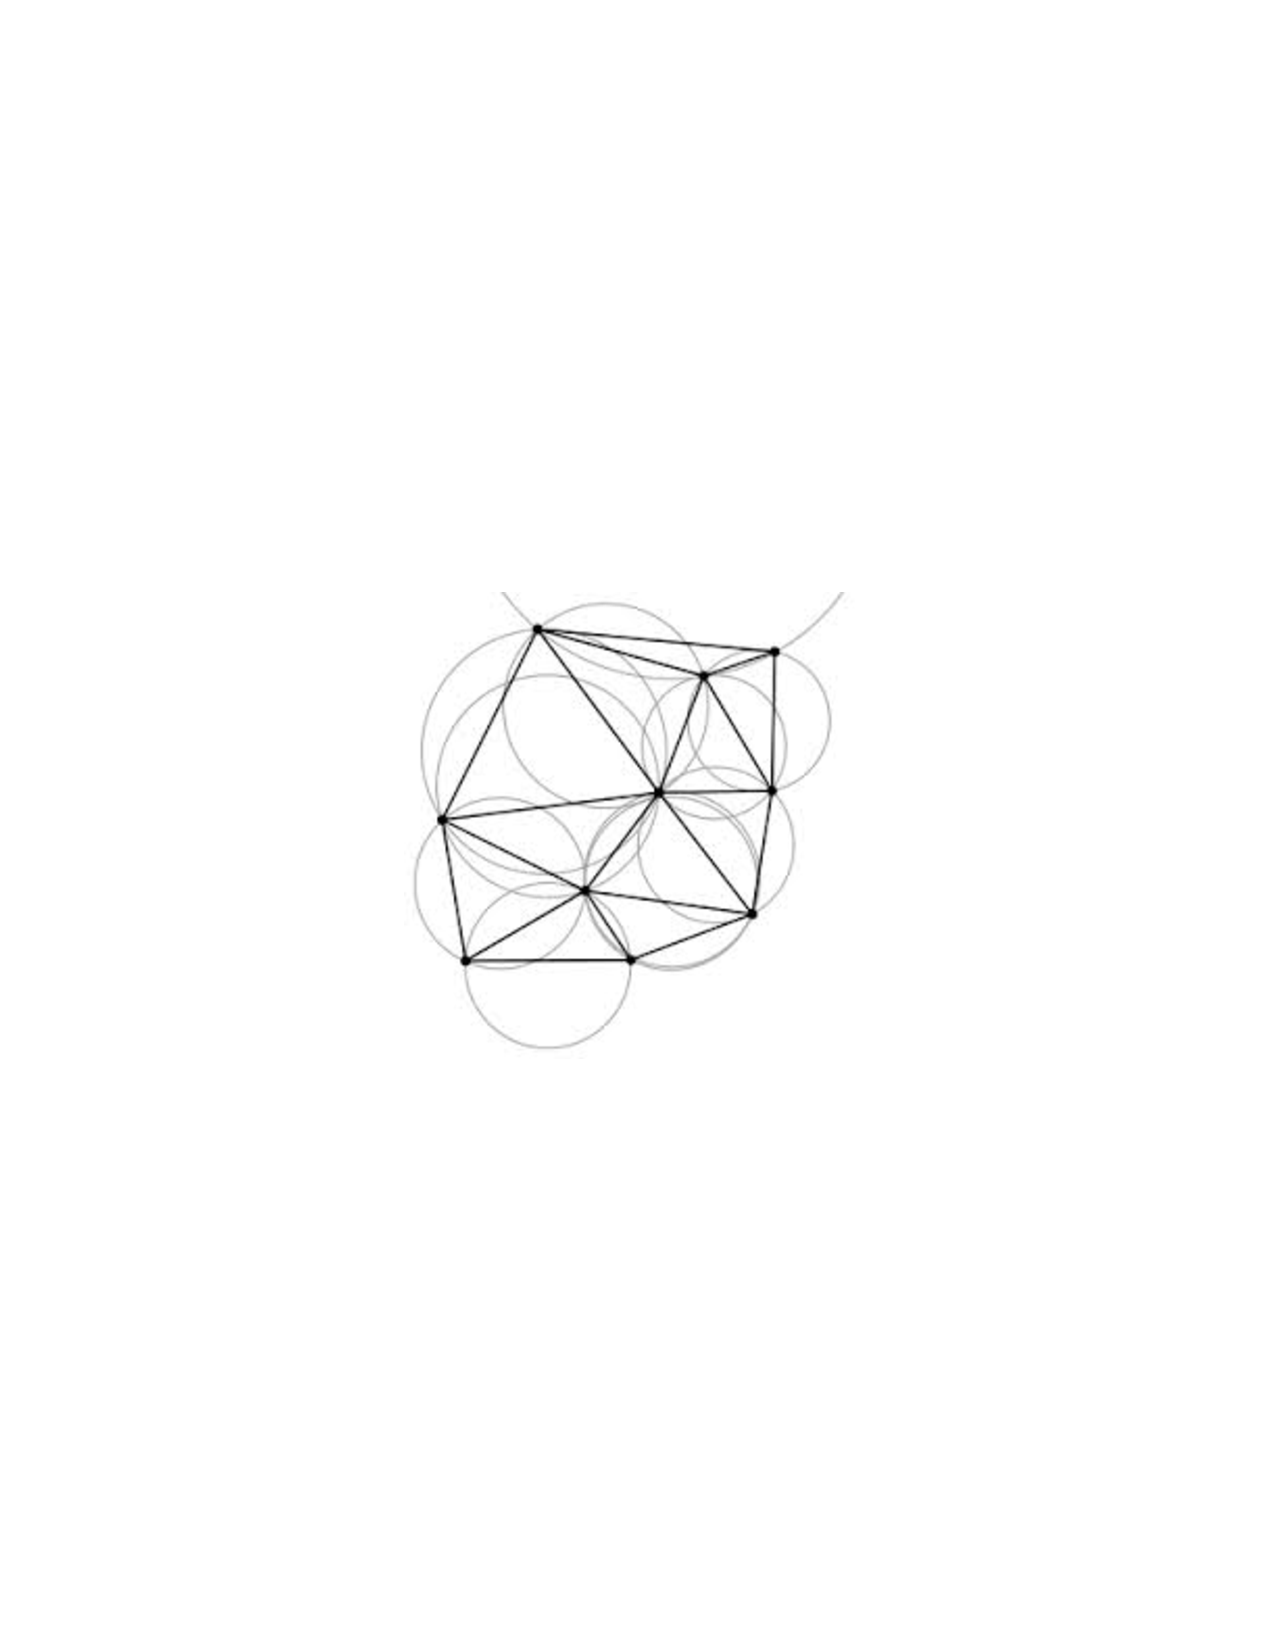
\includegraphics[width=2in]{DT1.pdf}
   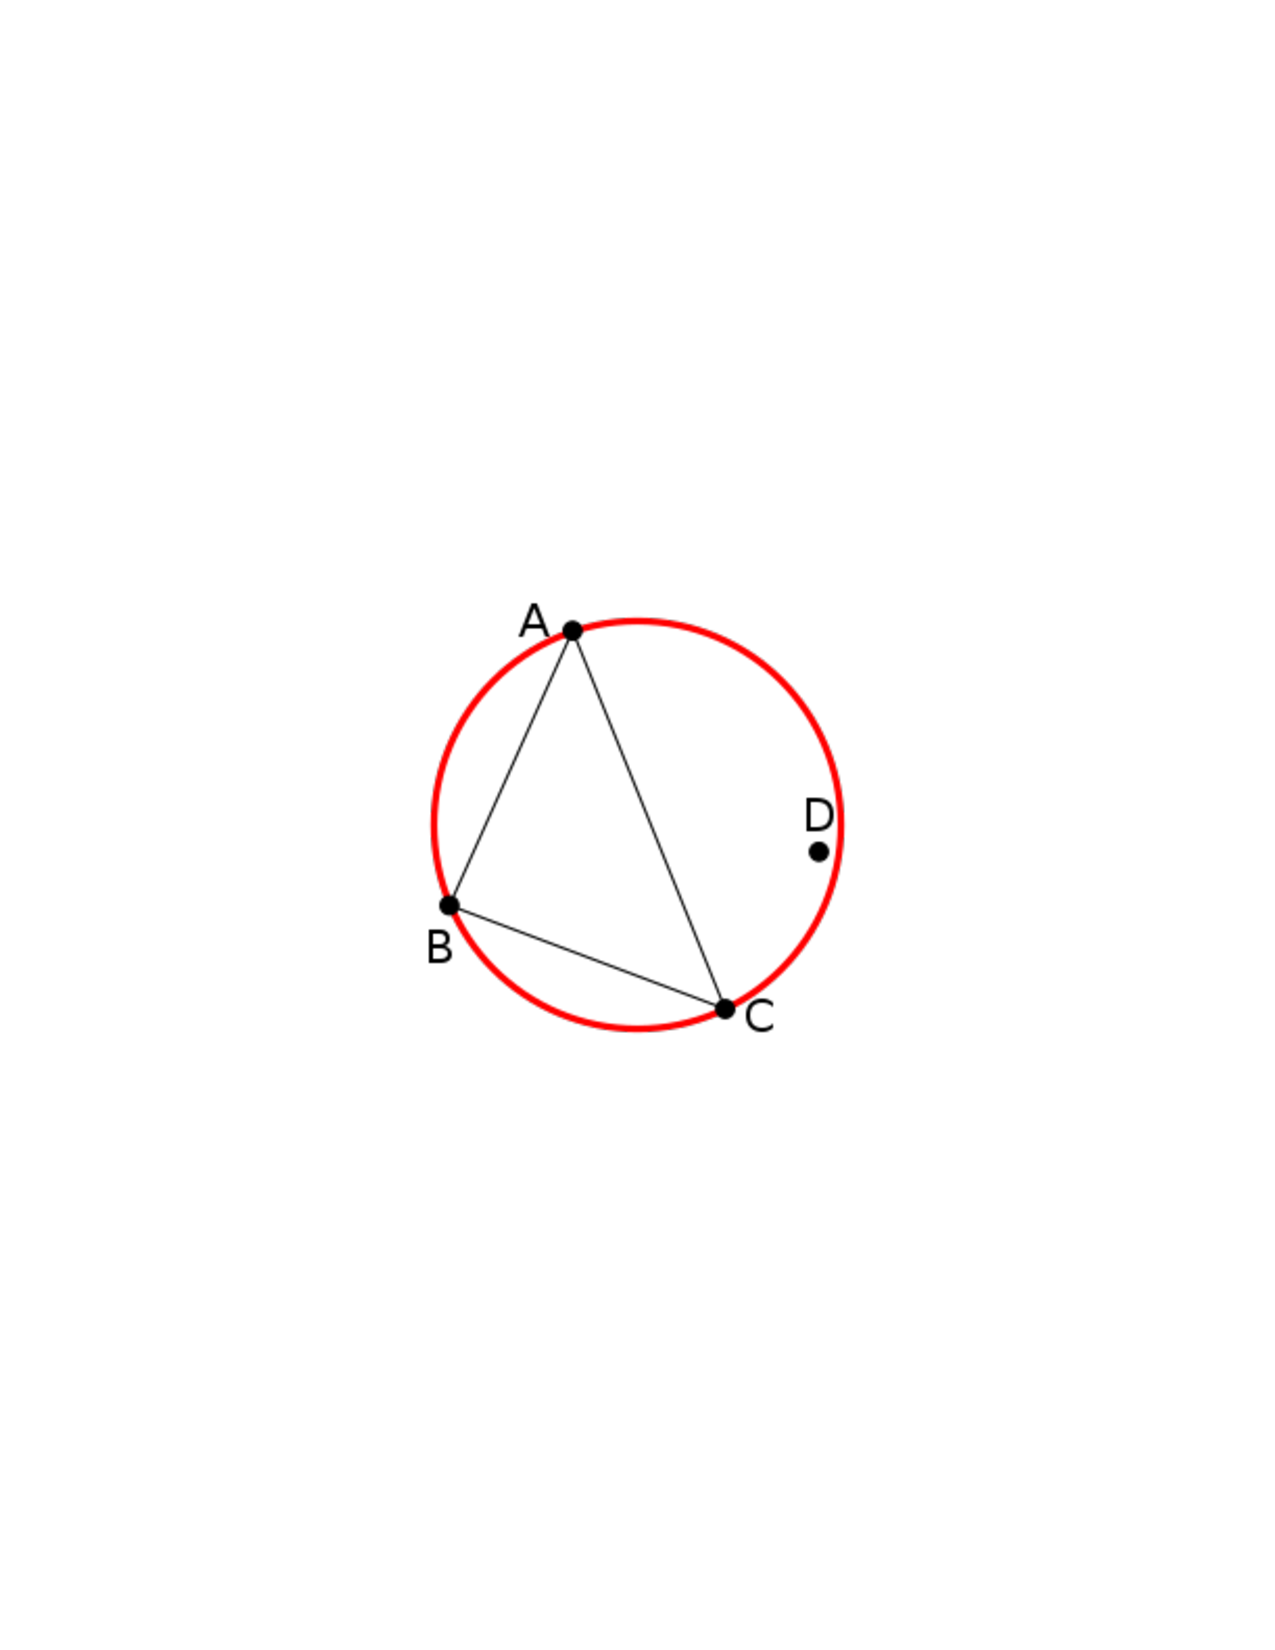
\includegraphics[width=2in]{NDT.pdf}
  \caption{Delaunay triangulation (left) Not a Delaunay triangulation (right) \label{DT}}
  \end{center}
\end{figure}

The discrete version of the Einstein-Hilbert action is the Regge action:

\begin{align}
  I_{R}=\frac{1}{8\pi G_{N}}\left(\sum\limits_{hinges}A_{h}\delta_{h}-\Lambda\sum\limits_{simplices}V_{s}\right)\label{equation:Regge-Action}
\end{align}

And the discrete version of the path integral is (after a Wick rotation:

\begin{align}
  \langle B|T|A\rangle=\sum\limits_{triangulations}\frac{1}{C(T)}e^{-I_{R}(T)} \label{CDT1}
\end{align}

Here, we take a sum over all inequivalent triangulations. In 1991 Pachner\cite{pachner_p.l._1991}, building on Alexander's work in the 1930s\cite{alexander_combinatorial_1930}
showed that elementary operations, now called Pachner moves, could transform a triangulation $T$ to another manifold $T'$ homeomorphic to $T$. The set of all inequivalent triangulations could be then be explored via a series of Pachner moves.\cite{gross_elementary_1992}

\Cref{CDT1} takes advantage of the distinctly causal nature of Causal Dynamical Triangulations. That is, the triangulations are foliated by hypersurfaces of distinct time.
Using this innovation allows an explicit calculation of the CDT action, which has been done for 2, 3, and 4 dimensions. The subject of this paper is the 3D action:

\begin{eqnarray*}
  I_{CDT}^{(3)} &=& 2\pi k\sqrt{\alpha}N_1^{TL} \\
    &+& N_3^{(3,1)}\left[-3k\text{arcsinh}\left(\frac{1}{\sqrt{3}
    \sqrt{4\alpha +1}}\right)-3k\sqrt{\alpha}\text{arccos}\left(\frac{2\alpha+1}
    {4\alpha+1}\right)-\frac{\lambda}{12}\sqrt{3\alpha+1}\right] \\
    &+& N_3^{(2,2)}\left[2k\text{arcsinh}\left(\frac{2\sqrt{2}\sqrt{2\alpha+1}}
    {4\alpha +1}\right)-4k\sqrt{\alpha}\text{arccos}\left(\frac{-1}{4\alpha+1}
    \right)-\frac{\lambda}{12}\sqrt{4\alpha +2}\right]\label{CDT2}
\end{eqnarray*}

Where $\alpha$ is the length of the timelike edges (spacelike edges are length 1), $k=\frac{1}{8\pi G_{N}}$, and $\lambda=k*\Lambda$.

To evaluate \Cref{CDT1}, we use the Metropolis-Hastings algorithm as follows:\\[-4ex]
\begin{enumerate}\addtolength{\itemsep}{-1.5ex}
\item Selection: Pick a Pachner move;  
\item Acceptance: Make that move with a probability of $a=a_1a_2$, where
\end{enumerate}
\vspace*{-1ex}

\begin{align}
  a_{1}=\frac{move[i]}{\sum\limits_{i}move[i]}
\end{align}

\begin{align}
  a_{2}=e^{\Delta I_{CDT}}
\end{align}

Note that we have divided out the partition function $\frac{1}{C(T)}$ in \Cref{CDT1}, which we didn't know how to evaluate anyway.

After thermalization, the Metropolis-Hastings algorithm gives us the distribution of triangulations for comoputing the path integral. We can then perform measures
on these representative ensembles to calculate properties such as spectral dimension.\cite{j._ambjorn_spectral_nodate,sotiriou_spectral_2011}

\section{Dynamical System}

To generate the causal sets used in our analysis, we created a Mathematica notebook
 that allowed us to select random points uniformly from a causal diamond in
Minkowski space, initially in four dimensions.   We calculated the Myrheim-Meyer dimension
and verified that it agreed with the dimension of of the background manifold in the  limit
of dense sprinklings.  As is evident from figure \ref{fig1}, this limit was already reached
with sprinklings of about 20 points, so we used this as a typical size.

\begin{figure}
\begin{center}
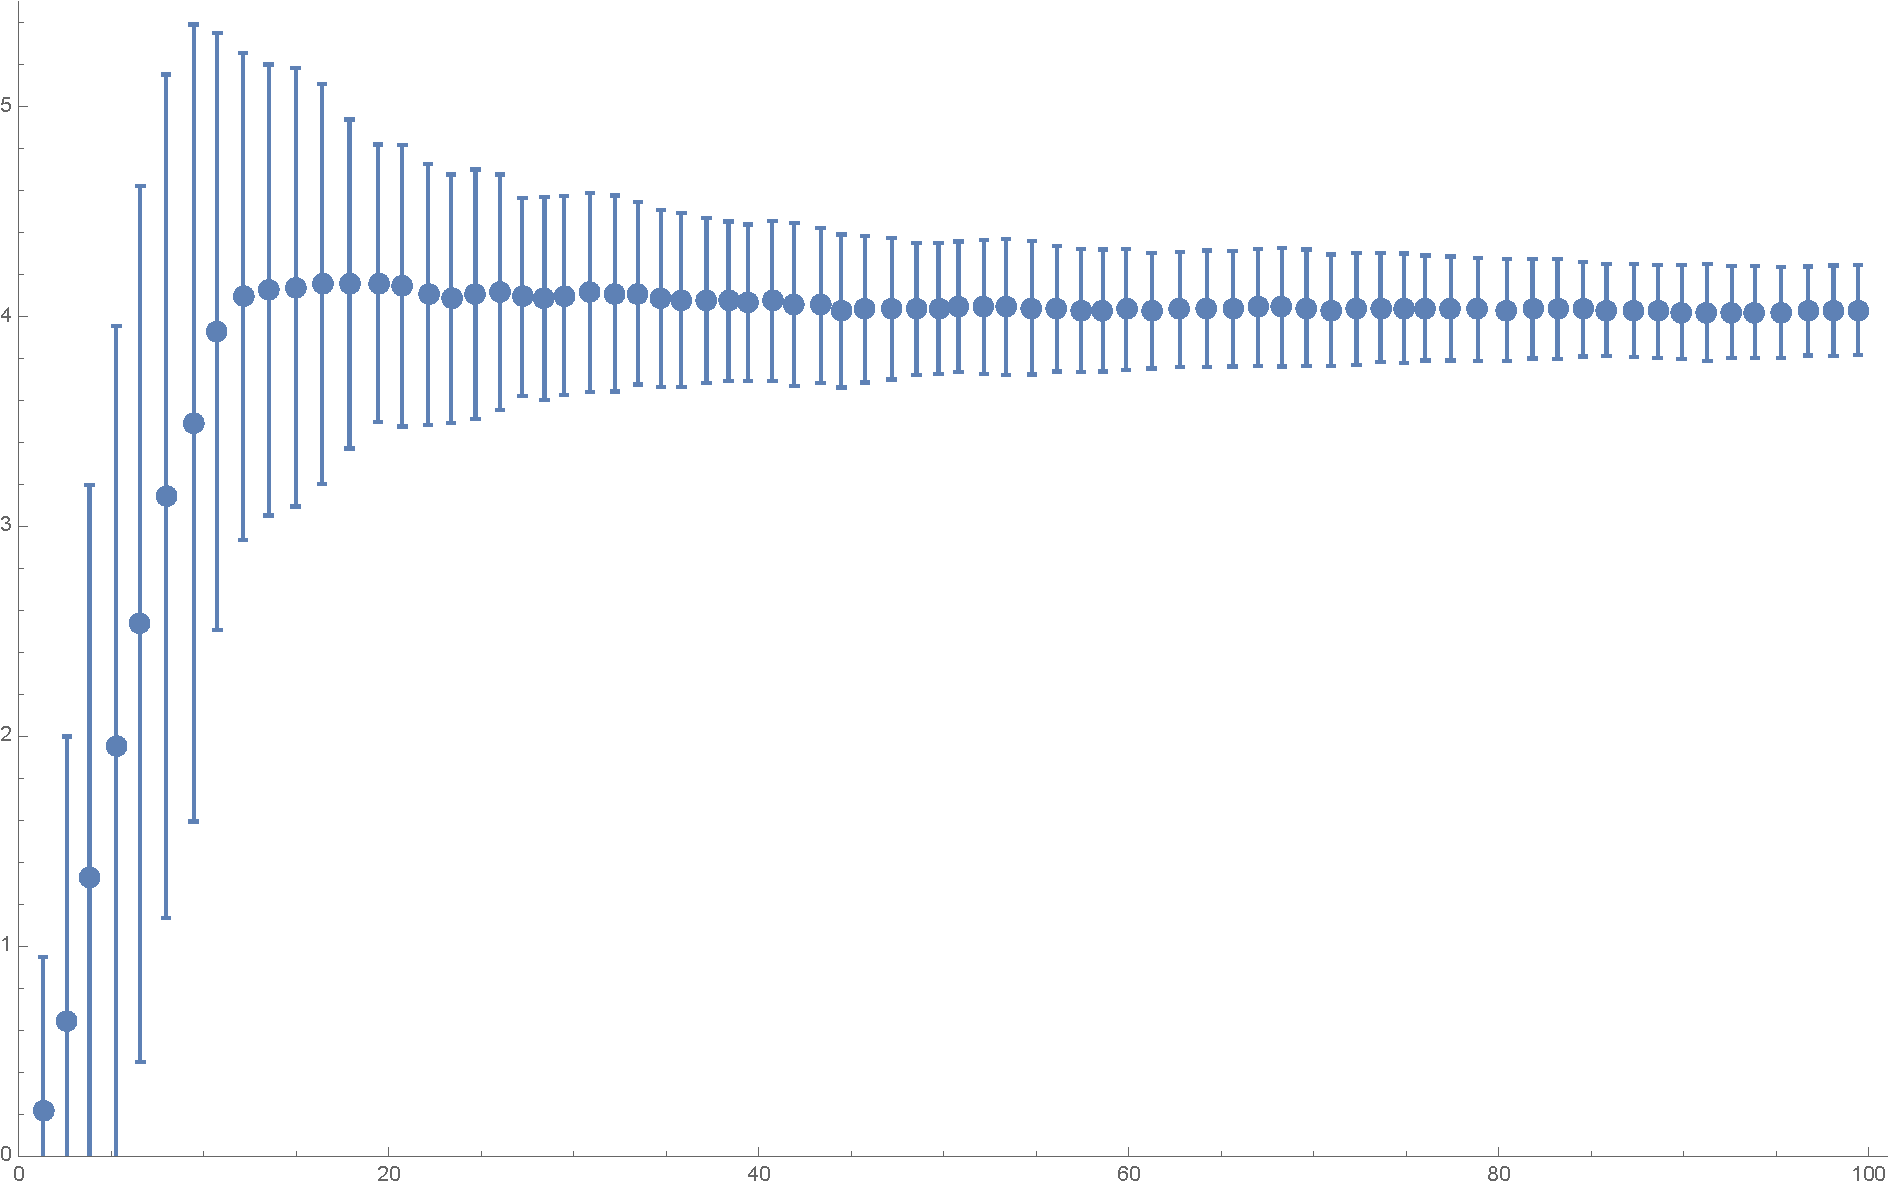
\includegraphics[height=2.5in]{CSDimRedLrg.pdf}
\caption{Myrheim-Meyer dimension for subsets of a relatively large causal set \label{fig1}}
\end{center}
\end{figure}

To investigate the dependence of dimension on volume, one must choose a way to
of select causal sets of ``small" volume.  Since the volume of a causal set is
determined by the number of points in the set, it is tempting to simply average
over all subsets containing a given number of points.  This can be misleading, though:
while such sets are ``small" if viewed outside the context of the background
spacetime, most of them do not come from a small region of the background spacetime,
but include points spread across a large region of the background manifold.   In
particular, two points with a lightlike separation can be ``adjacent'' in a causal set
even if they are widely separated in spacetime.

As an alternative, for each of our sprinklings we considered successively smaller sub-diamonds
in the background spacetime.  The points in each sub-diamond constitute a new causal
set, whose volume and Myrheim-Meyer dimension we computed.  We repeated the
process for 10,000 sprinklings, and then averaged the dimension at
each volume.  We initially applied this analysis to four-dimensional Minkowski space,
but subsequently repeated it for $d=3$ and $d=5$.

As noted above, the Myrheim-Meyer dimension is not well-defined for single points or
causal sets with no edges.  While this concern is unimportant for large causal sets, it
must be confronted for the very small sets  we are interested in.  We explored
two reasonable possibilities: taking the volume of an isolated point to be zero (they are,
after all, single points) or dropping edgeless causal sets from our counting (they
are causally disconnected from the rest of spacetime).

\section{Results}

In each of the background dimensions we studied, we found that dimensional reduction
does indeed occur as the volume decreases.   As shown in figures \ref{fig2}--\ref{fig4},
the process appears to be smooth, but has a rather abrupt onset.  The
transition to lower dimension starts at a volume of approximately $V=8$ points in
three dimensions, $V=16$ points in four dimensions, and $V=22$ points in five
dimensions.\footnote{Fractional volumes appear in the graphs because at a given
background volume in Minkowski space, causal sets with varying numbers of points
may be present.}

At volumes above the transition, the Myrheim-Meyer dimension remains stable and
equal to the dimension of the background Minkowski space.  Below the transition,
the decrease is quite rapid.  For each of the background dimensions we considered,
the minimum Myrheim-Meyer dimension falls to $d_M\approx 0$ if edgeless causal
sets are taken to have dimension zero, and $d_M\approx 2$ if they are omitted.
We can understand the latter result by noting that the smallest causal set with an
edge---two points with one relation---has a Myrheim-Meyer dimension of two.

Figures \ref{fig2}--\ref{fig4} show $1\, \sigma$ error bars.  We believe these are not
a result of poor statistics, but are rather a consequence of our definition of
volume.  A causal diamond of a given volume in a background Minkowski space can
contain many different causal sets, which will not all have identical Myrheim-Meyer
dimensions.  This leads to a genuine statistical fluctuation in dimension, especially
at small volumes.

The end point $d_M\approx 2$ is reminiscent of the behavior seen in other
investigations of quantum gravity.  More precisely, when edgeless causal
sets are discarded, we find a minimum dimension of $d_M = 2.08 \pm .26$ in three
background dimensions, $d_M = 2.13 \pm .39$ in four background dimensions, and
$d_M = 2.19 \pm .40$ in five background  dimensions.  It would be interesting to
understand the fluctuations better, especially since a few other approaches to
quantum gravity suggest a minimum dimension of $3/2$

We would also like to understand what determines the scale at which dimensional
reduction sets in.  For three and four background dimensions, the transition seems to
occur at a characteristic length of about twice the sprinkling length---that is,
$V\sim 2^d$ points---but this pattern appears to break down for background
 dimension five.  We also plan to investigate the behavior of another standard
dimensional estimator, midpoint scaling dimension 

Ideally, we would like to do more.  The results we have presented here have the
awkward feature of relying on the background Minkowski space to define the
small regions whose dimension we measure.  This was necessary to avoid picking
out causal subsets that were ``small'' in the sense of having few points, but
``large'' in the sense of occupying a highly extended region.  Recently, some
progress has been made in defining ``local'' regions entirely in the context of
causal sets, without reference to any background .  It might be
possible to use this work to investigate dimensional reduction more intrinsically.



\begin{figure}
\begin{center}
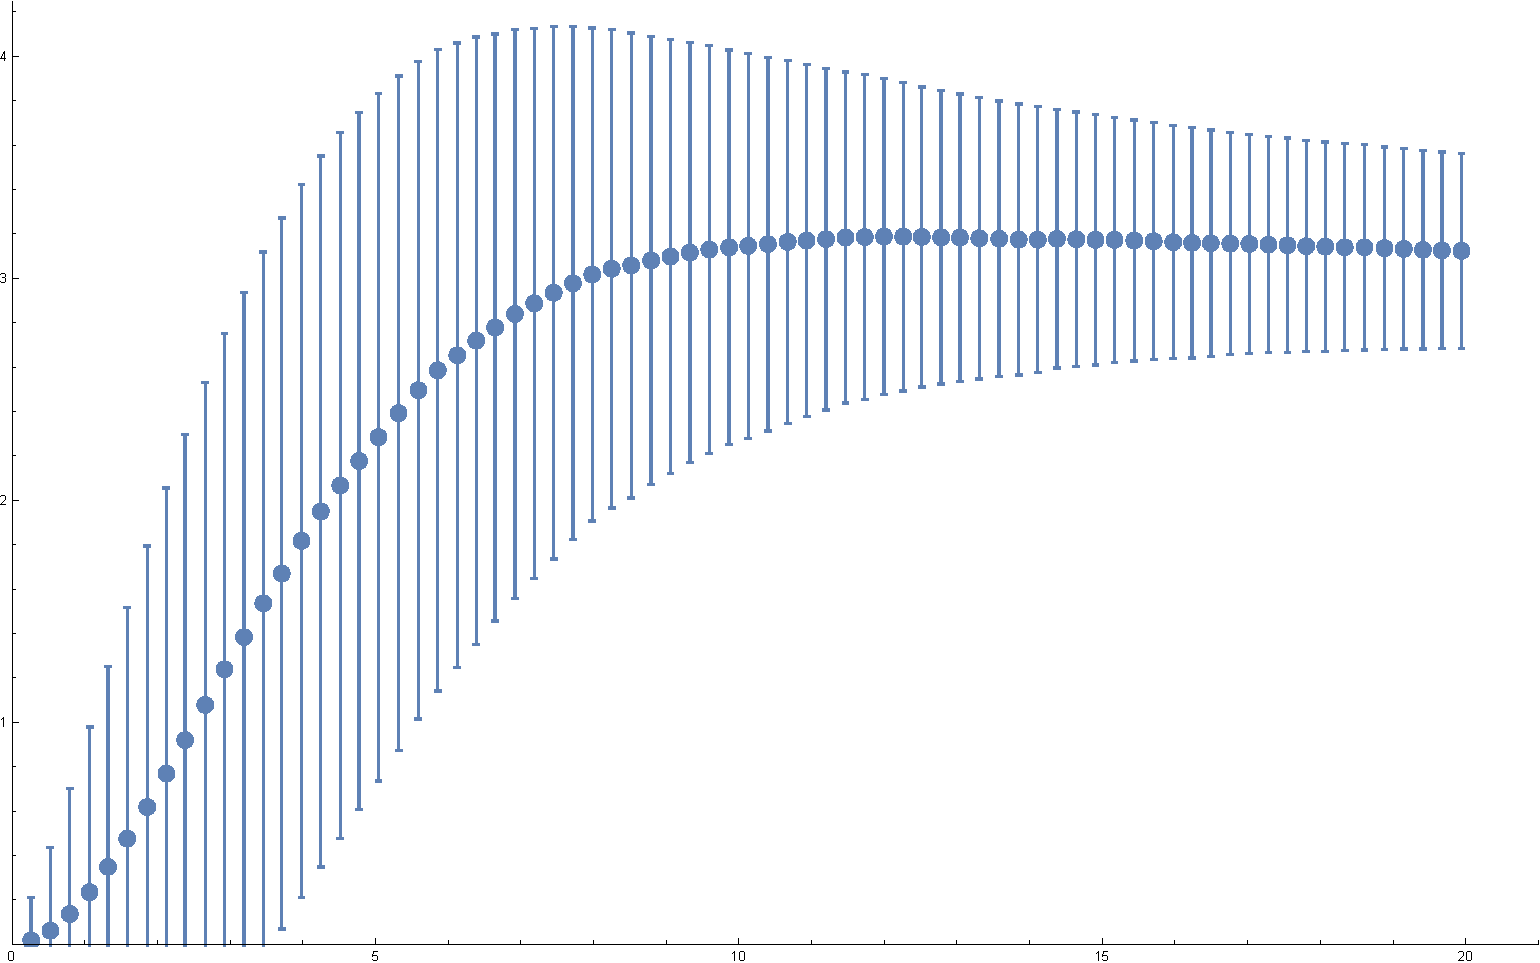
\includegraphics[width=3.15in]{CSDimRed3D.pdf}
 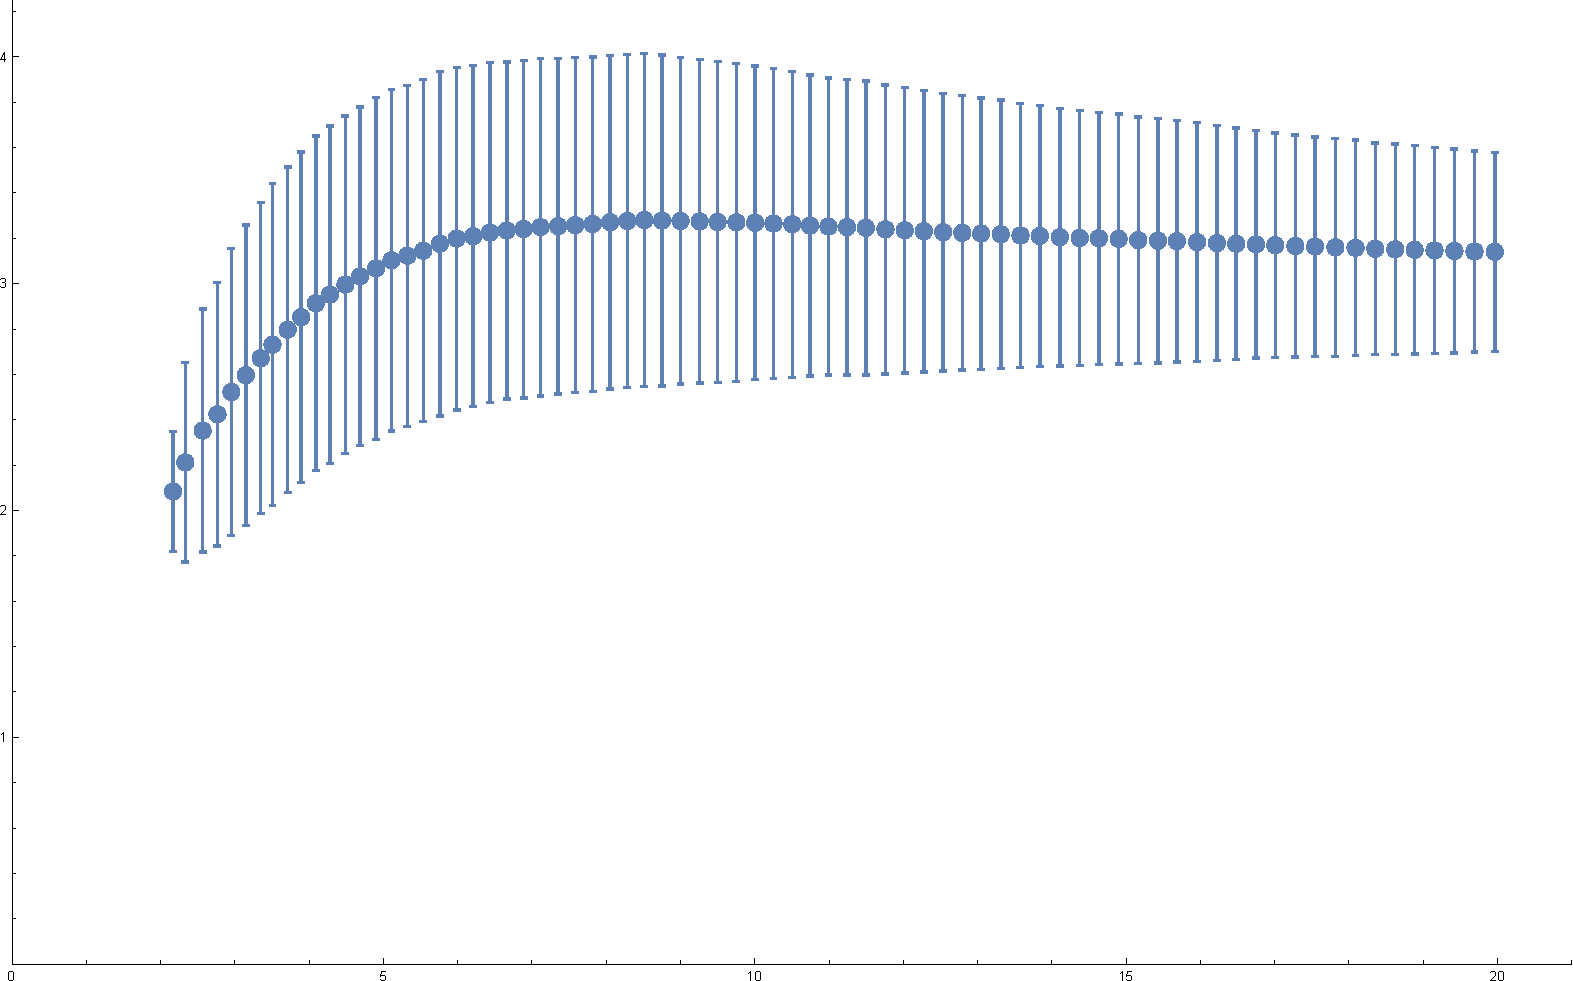
\includegraphics[width=3.15in]{CSDimRed3D2.pdf}
\caption{Myrheim-Meyer dimension in a three-dimensional background,
with edgeless sets counted as dimension zero (left) or omitted (right) \label{fig2}}
\end{center}
\begin{center}
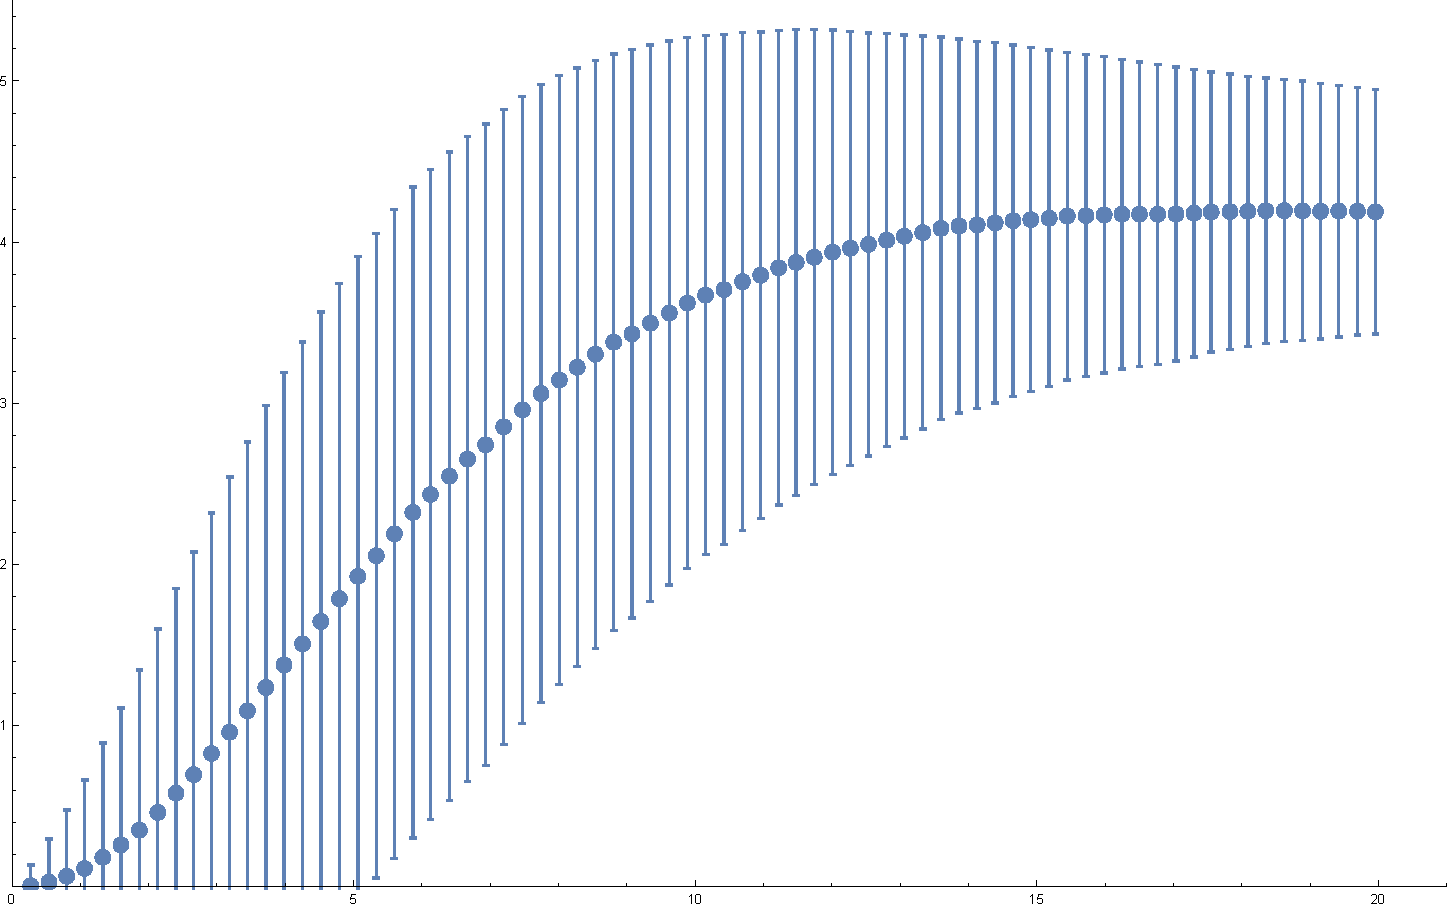
\includegraphics[width=3.15in]{CSDimRed.pdf}
 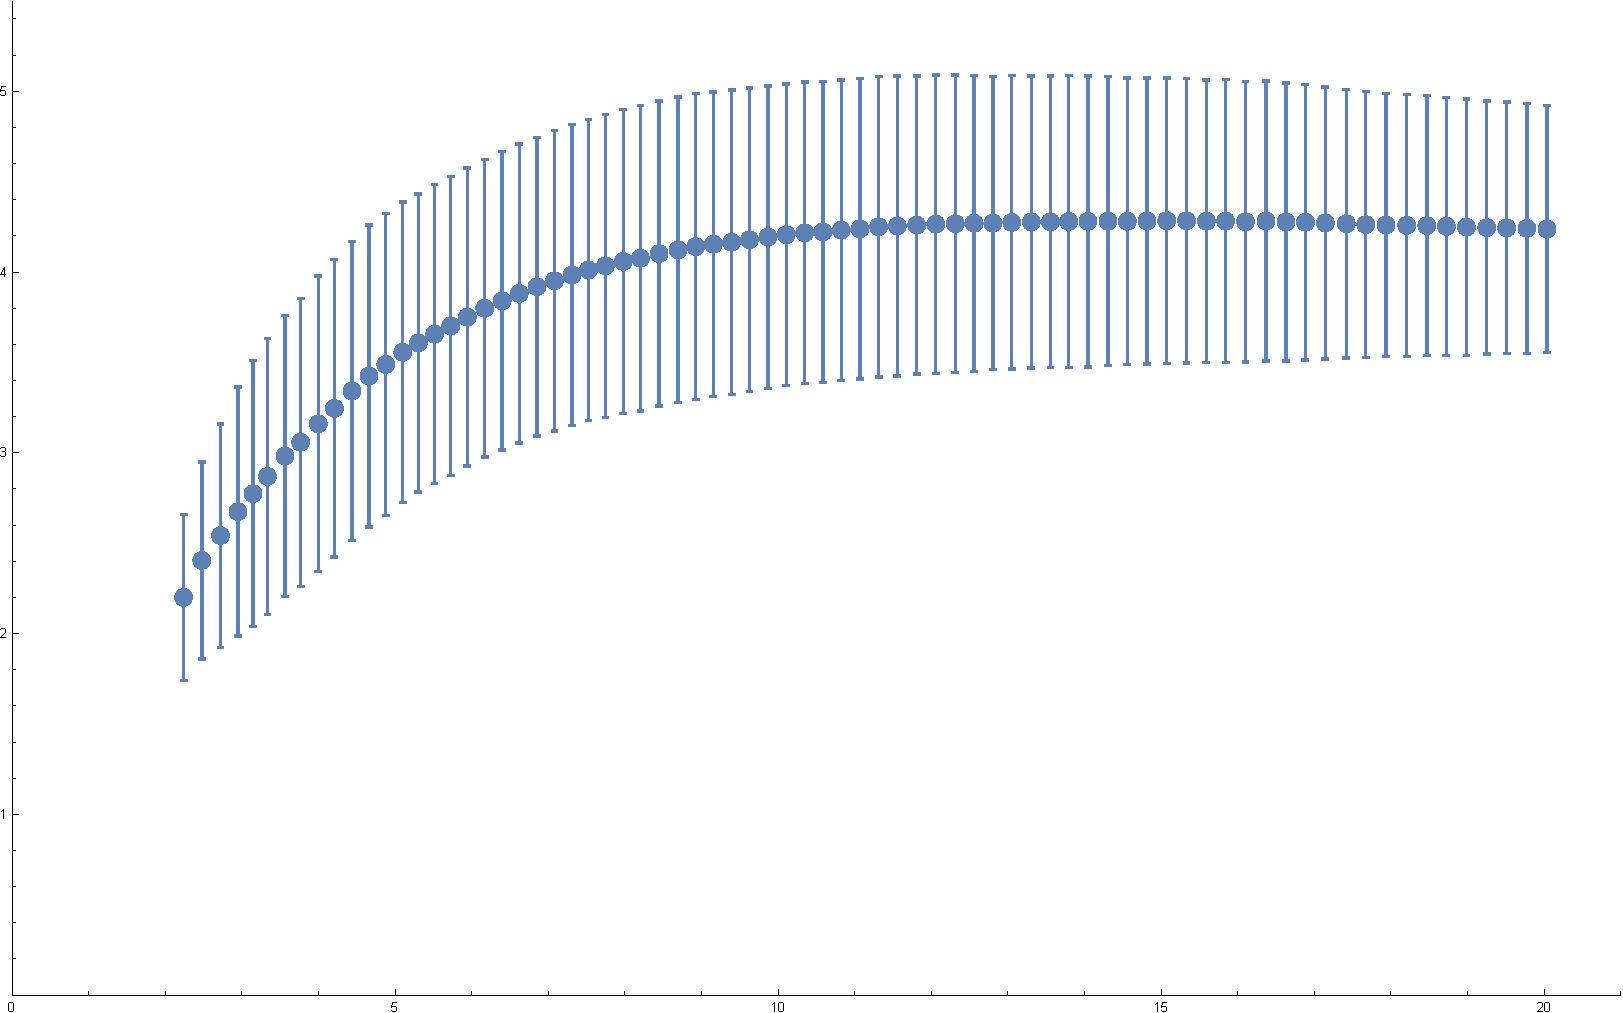
\includegraphics[width=3.15in]{CSDimRed2.pdf}
\caption{Myrheim-Meyer dimension in a four-dimensional background,
with edgeless sets counted as dimension zero (left) or omitted (right) \label{fig3}}
\end{center}
\begin{center}
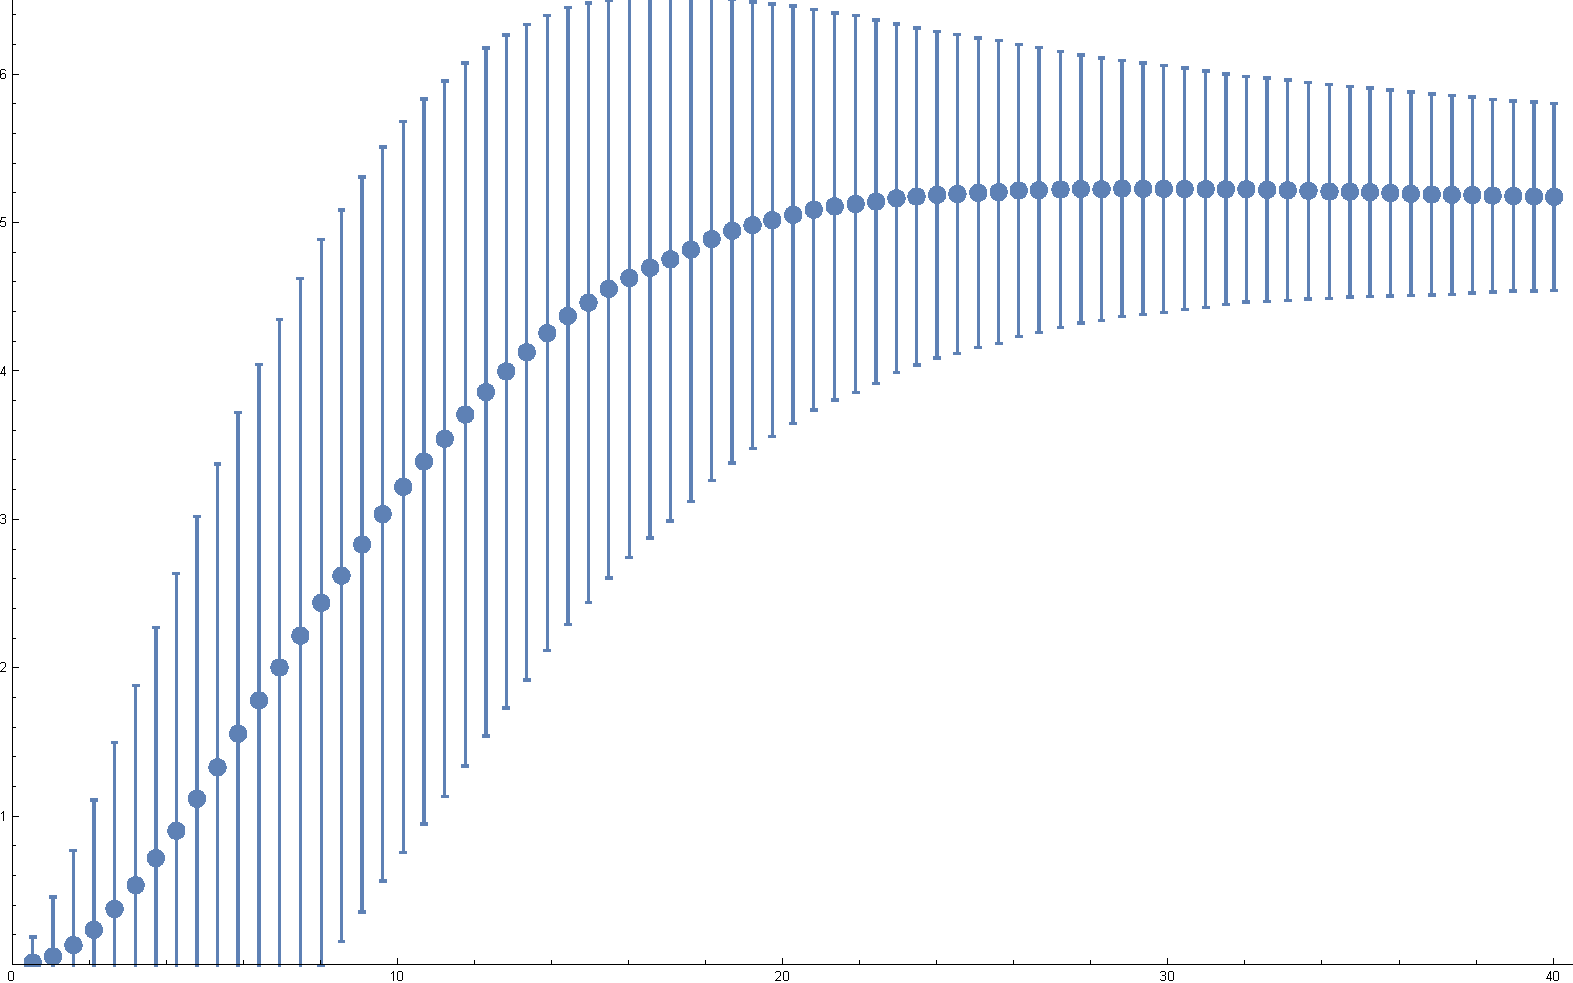
\includegraphics[width=3.15in]{CSDimRed5D.pdf}
 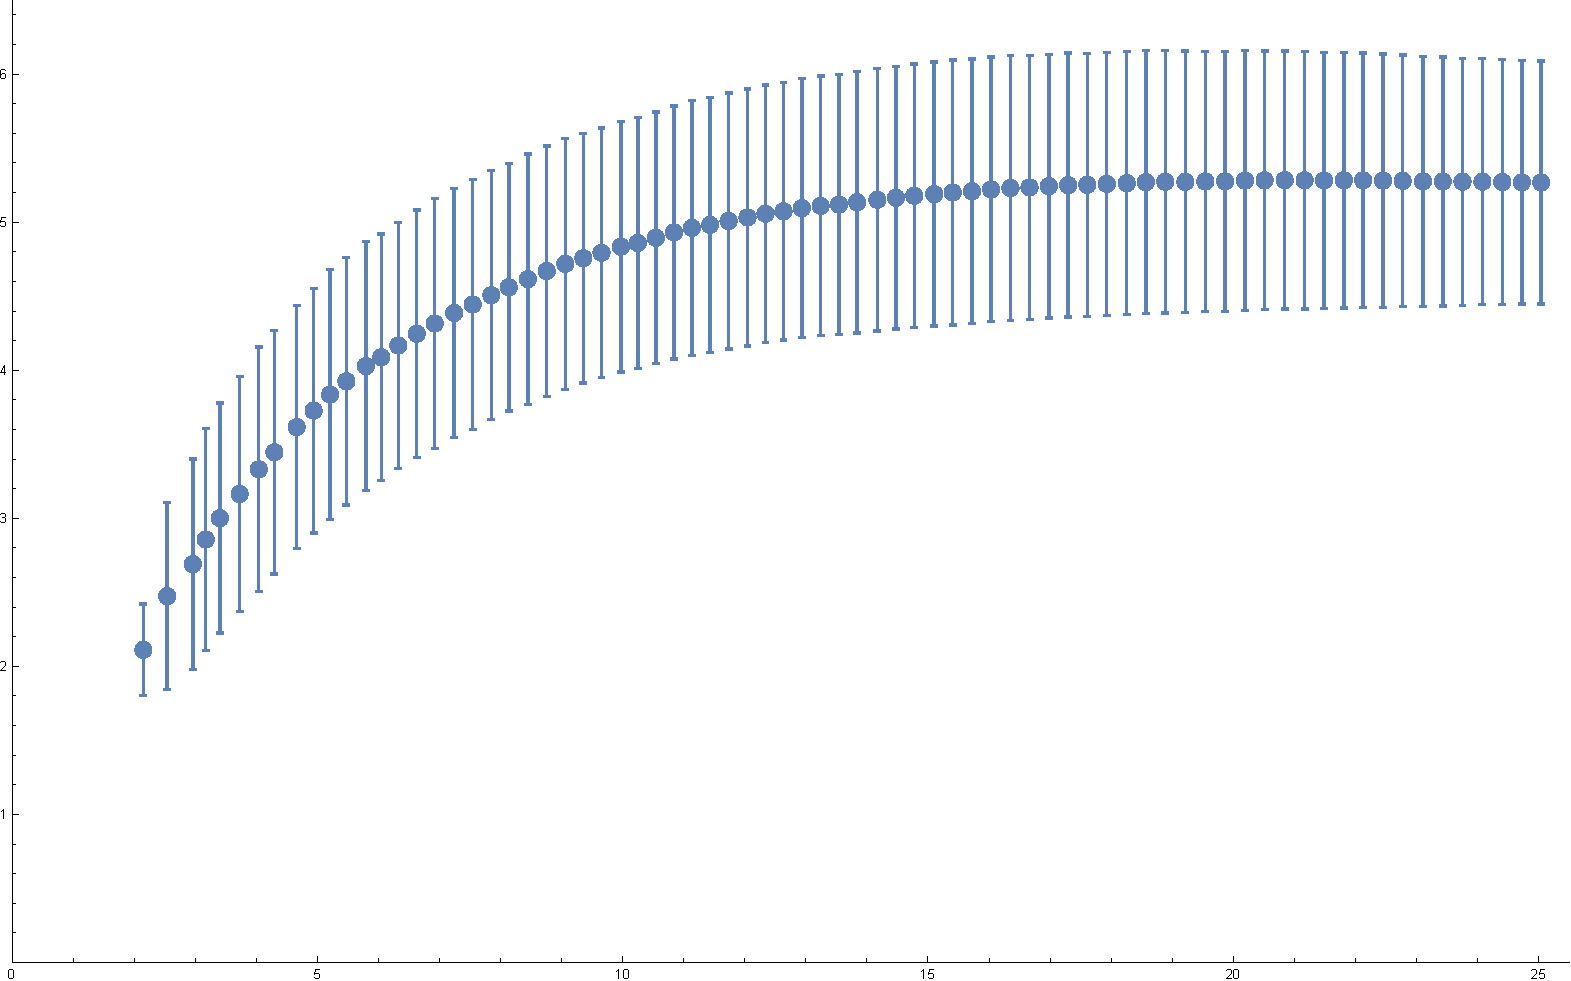
\includegraphics[width=3.15in]{CSDimRed5D2.pdf}
\caption{Myrheim-Meyer dimension in a five-dimensional background,
with edgeless sets counted as dimension zero (left) or omitted (right) \label{fig4}}
\end{center}
\end{figure}

\newpage

\vspace{1.5ex}

\bibliographystyle{ieeetr}
\bibliography{EfficientCDT.bib}
\end{document}
